\documentclass[12pt,twoside]{article}
\usepackage{hyperref} 
%\usepackage{minted}
\usepackage{verbatim}
\usepackage{graphicx}

\newcommand{\doctitle}{%
Hamiltonian Cycles}

\pagestyle{myheadings}
\markboth{\hfill\doctitle}{\doctitle\hfill}

\bibliographystyle{siam}

\addtolength{\textwidth}{1.00in}
\addtolength{\textheight}{1.00in}
\addtolength{\evensidemargin}{-1.00in}
\addtolength{\oddsidemargin}{-0.00in}
\addtolength{\topmargin}{-.50in}

\hyphenation{in-de-pen-dent}

\title{\textbf{\doctitle}\\
CS7081 Final Project Report - Group 2}

\author{Jayanth Dungavath \hspace{.1cm}\\Madhav Lolla\hspace{.1cm}\\Soumya Nayak\hspace{.1cm}\\Kranthi Pamarthi }
%\author{Prudhvi Shedimbi}
%\author{Madhulika Alugubelli}

\begin{document}
\maketitle
\pagebreak



\hfill \break
\hfill \break
\hfill \break
\hfill \break
\hfill \break
\hfill \break
\hfill \break
\hfill \break
\hfill \break
\hfill \break
\hfill \break
\hfill \break
\hfill \break
\hfill \break
\hfill \break
\hfill \break
\hfill \break
\hfill \break
\hfill \break
\hfill \break
\hfill \break
\hfill \break
\hfill \break
\hfill \break
\hfill \break
\hfill \break
\pagebreak

\tableofcontents
%\thispagestyle{empty}


\hfill \break
\hfill \break
\hfill \break
\hfill \break
\hfill \break
\hfill \break
\hfill \break
\hfill \break
\hfill \break
\hfill \break
\hfill \break
\hfill \break
\hfill \break
\hfill \break
\hfill \break
\hfill \break
\hfill \break
\hfill \break
\hfill \break
\hfill \break
\hfill \break
\hfill \break
\hfill \break
\hfill \break
\hfill \break
\hfill \break
\hfill \break
\pagebreak

%\graphicspath{ {/Users/jayanthdeejay/Desktop/} }


\section{Introduction}
A Hamiltonian cycle is a graph cycle through a graph that visits each node exactly once \emph{(Skiena 1990, p. 196)}. A graph possessing a Hamiltonian cycle is said to be a Hamiltonian graph. The Hamiltonian cycle is named after Sir William Rowan Hamilton, who devised a puzzle in which such a path along the polyhedron edges of an dodecahedron was sought (the Icosian game). In general, the problem of finding a Hamiltonian cycle is NP-complete \emph{(Karp 1972; Garey and Johnson 1983, p. 199)}, so the only known way to determine whether a given general graph has a Hamiltonian cycle is to undertake an exhaustive search. Rubin (1974) describes an efficient search procedure that can find some or all Hamilton paths and circuits in a graph using deductions that greatly reduce backtracking and guesswork. A probabilistic algorithm due to Angluin and Valiant (1979), described by Wilf (1994), can also be useful to find Hamiltonian cycles and paths.
\hfill \break
\hfill \break
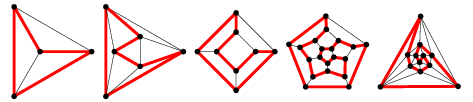
\includegraphics[width=\textwidth]{1.png}
\hfill \break
All Platonic solids are Hamiltonian \emph{(Gardner 1957)}, as illustrated above (top view of the solids). For this particular project, we have studied various research papers online related to Hamiltonian Cycles, their behavior and applications.
\hfill \break
\section{Research}
In this section, we briefly cover the papers that we have studied while working on this project. The study
of Hamiltonicity has mainly been concerned with looking for simple sufficient conditions implying
Hamiltonicity. One of the most important results in this direction is Dirac's theorem asserting that
every n-vertex graph, \begin{test} n \leq 3 \end{test} of minimum degree at least n/2 contains a Hamilton cycle. In the paper \emph{Compatible Hamilton cycles in Dirac graphs} (2014) [1], authors have proved that there is a constant \begin{test} \mu > \end{test}  0 such that for every \begin{test} \mu \end{test}n-bounded incompatibility system F over a n-vertex Dirac graph G, there exists a Hamilton cycle compatible with F. In this context, they have defined a \emph{Dirac graph} as an n-vertex graph of minimum degree at least n/2. \\ \\
In another paper titled \emph{Robust hamiltonicity of random directed graphs} (2014) [2], authors have worked on hamiltonicity of random directed graphs. The theorems of Dirac and Ghouila-Houri state that the local resilience of the complete graph and digraph with respect to Hamiltonicity is 1/2. Lee and Sudakov (2012) proved that the local resilience of a random graph with edge probability p = \emph{w} (log n/n) with respect to Hamiltonicity is 1/2\begin{test} \pm \end{test} o(1). For random directed graphs, Hefetz, Steger and Sudakov (2014+) proved an analogue statement, but only for edge probability p = \emph{w} (log n/\begin{test}\sqrt{n}\end{test}). Authors in this paper have worked on improving the probability to p = \emph{w} (log\begin{test}^{8}\end{test}   n/n), which is optimal up to the polylogarithmic factor. \\ \\
Asghar Asgharian Sardroud, in a paper titled \emph{An approximation algorithm for the longest cycle problem in solid grid graphs} (2015) [3], presented linear-time constant-factor approximation algorithm that, given a 2- connected, n-node solid grid graph, can find a cycle containing at least two third of its vertices. \\ \\
After reading few other papers related to Hamiltonian cycles, we chose to study it's applications. One of the famous applications of Hamiltonian cycles is Traveling Salesman Problem (TSP). Ricardo Fukasawa, Allan Sapucaia Barboza and Alejandro Toriello have presented a paper titled \emph{A Comparison of Bounds for the Traveling Salesman Problem} (2015) [4], in which they considered two different families of lower bounds for the \emph{traveling salesman problem} (TSP). One of them is a recently proposed \emph{approximate linear programming} (ALP) bound, the other is obtained by adapting a bound from related routing problems called the \emph{branch-cut-and- price} (BCP) family. They have showed that the two families ALP and BCP are incomparable both theoretically and empirically. \\ \\
Finally we read the paper by Brad Woods, Abraham Punnen and Tamon Stephen titled \emph{Linear time algorithm for the 3-neighbor traveling salesman problem on Halin graphs and extensions} (2015) [5]. They have define a restricted version of quadratic traveling salesman problem, the k- neighbour TSP (TSP(k)), and gave a linear time algorithm to solve TSP(k) on a Halin graph for \begin{test} k \leq 3 \end{test}. \\ \\
\begin{center}
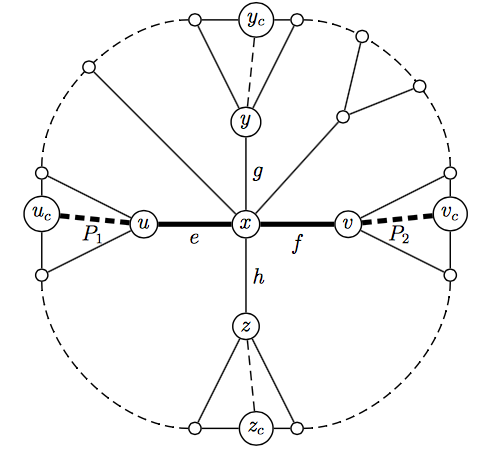
\includegraphics[scale=.4]{2.png}\\
Halin Graph [5]
\end{center}

\section{Environment}
\begin{itemize}
    \item \textbf{OS}: Elementary OS Luna
    \item \textbf{Languages}: Python 3.0, C
    \item \textbf{Processor}: Intel Core 2 Duo, 2.2 GHz
    \item \textbf{Memory}: 4GB 800 MHz DDR2 SDRAM
    \item \textbf{Editor}: Emacs
    \item \textbf{Documentation}: TeXShop (Mac OS X)
\end{itemize}

\section{Algorithms}
We have investigated the following approaches and algorithms for this particular project.
\begin{itemize}
    \item Brute force algorithm
    \item Greedy method (Solving for Hamiltonian path)
    \item Backtrack method (solving for Hamiltonian cycle)
\end{itemize}
\subsection{Brute Force Algorithm:}
A random graph with n nodes will need (n-1)! operations to find the path. \\
Time Complexity: O(n!) \\
\textbf{Advantages:} Gives exact solution\\
\textbf{Disadvantages:} Complexity increases with increase in number of vertices. It is slow. \\

\begin{center}
\begin{tabular}{|r|l|}
  \hline
  Number of Vertices & Number of Cyclic Paths \\
  \hline
  5 & 24 \\
  6 & 120 \\
  7 & 720 \\
  8 & 5040 \\
  \hline
\end{tabular}
\end{center}

\subsection{Greedy Algorithm:}
The graph traverses based on the nearest neighbor available. A parallel approach was followed and idea taken from Kocay's Multipath algorithm. In the first iteration all the nodes are considered as individual segments. Then the nodes will form edges with nodes with different degrees. The segments thus formed will be concatenated. An optimization was It gave also used on the greedy method to find hamiltonian path faster. Rather than two segments, four segments are considered. The basic idea is to rearrange the path it is taking in hope of landing on a better solution.

\begin{center}
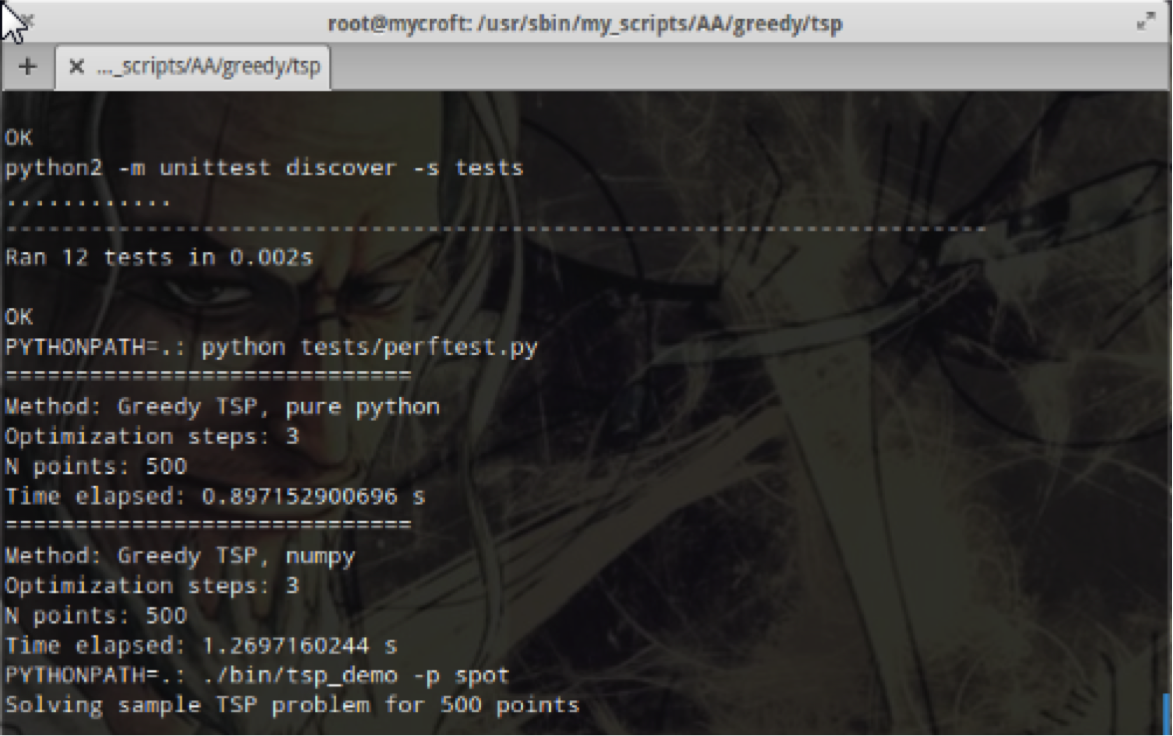
\includegraphics[width=\textwidth]{4.png}\\
Time elapsed to deduce a Hamiltonian path in a graph
\end{center}

\subsection{Backtrack Algorithm:}
We have used Kocay's multi path algorithm taken from Basil Vindergriend's master's thesis, 1998, Edmonton, Alberta. This particular algorithm uses exhaustive search to find a hamiltonian cycle. Key feature of this algorithm are the pruning techniques to reduce search space. Instead of one path, this algorithm maintains a set of paths. \\ \\
\textbf{Working}
\begin{itemize}
    \item The first segment is a randomly selected edge
    \item Whenever it finds a forced edge, that edge becomes a new segment    
    \item At each stage of the search, algorithm selects a random endpoint of a random segment to extend the partial solution
    \item If a�node has�two degree 2 neighbors, then all the�additional edges�incident on this node�can be deleted
\end{itemize}
Pruning Techniques depend on the partial solution available at each stage. Looking for small cut sets which when removed produces more components than the size of the cut set. If such a set exists, then hamilton path cannot exist. \\ \\
\textbf{Assumptions and relaxations:}
\begin{itemize}
    \item Space complexity of HP problems is at the worst polynomial
    \item Totally space inefficient algorithms will be \begin{test}O(n^2)\end{test}
    \item Since this wont be any limitation for hardware storage available now, our algorithms� are evaluated only on looking for the hamilton path
    \item An algorithm is deemed success if at least one hamilton path exists
\end{itemize} \\ \\
\textbf{Observations:}
\begin{center}
\begin{tabular}{|l|c|r|}
  \hline
  Experiment & \% Hamiltoninan graph & Algorithm success \\
  \hline
  Kocay's & 24\% &100\%  \\
  Greedy & NA & 100\% \\
  Greedy Opt. & NA & 100\% \\
  Brute force & NA^{*} & NA^{*} \\
  \hline
\end{tabular}
\end{center} \\
*The experiments were carried on graphs with a minimum of 500 nodes. So brute force was performed on a dataset of 8 points. In all the above cases, the algorithm worked and a hamilton path was found out. We observed that the time to find hamiltonian path in a bidirectional graph is faster than the uni directional graph. \\ \\
\textbf{Time:}
\begin{center}
\begin{tabular}{|r|l|}
  \hline
  Algorithm & Time to find single path \\
  \hline
  Greedy & 0.343062s \\
  Greedy with Numpy & 0.622528s \\
  Greedy opt. (3) & 0.8971529s \\
  Greedy opt. (3) with Numpy & 1.2697160s \\
  Kocay's & 0.6751004s \\
  Brute Force & NA \\
  \hline
\end{tabular}
\end{center}
\hfill \break
\hfill \break
\hfill \break
\hfill \break
\hfill \break
\hfill \break
\hfill \break
\hfill \break
\subsection{Resultant Hamiltonian paths:}
\begin{center}
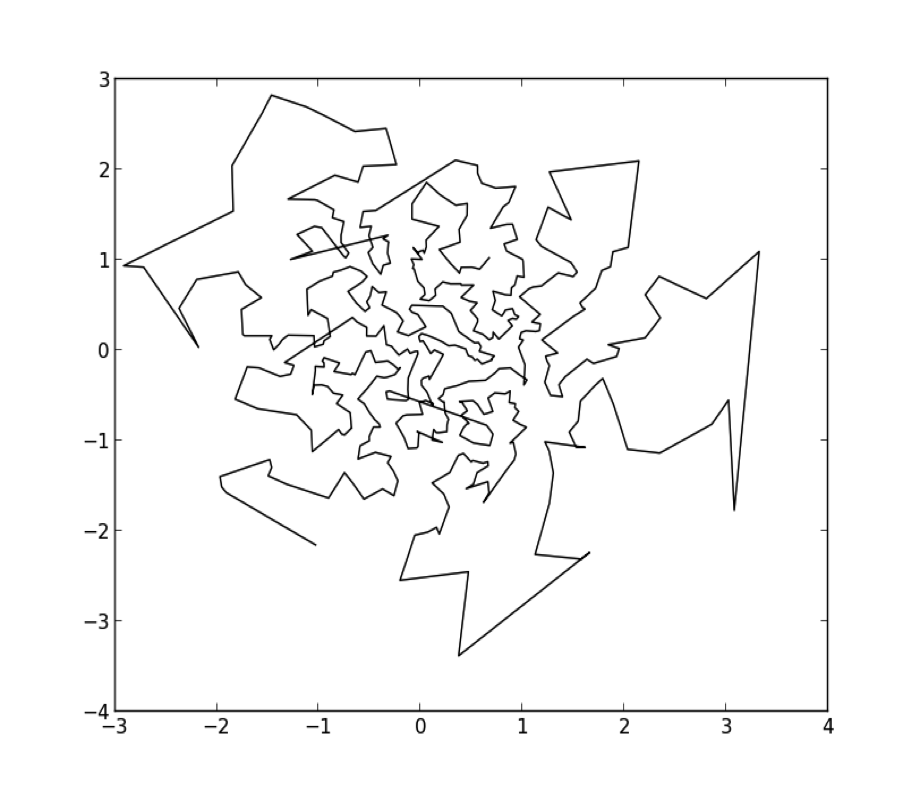
\includegraphics[scale=.6]{5.png}\\
Greedy 0 optimization
\end{center}
\begin{center}
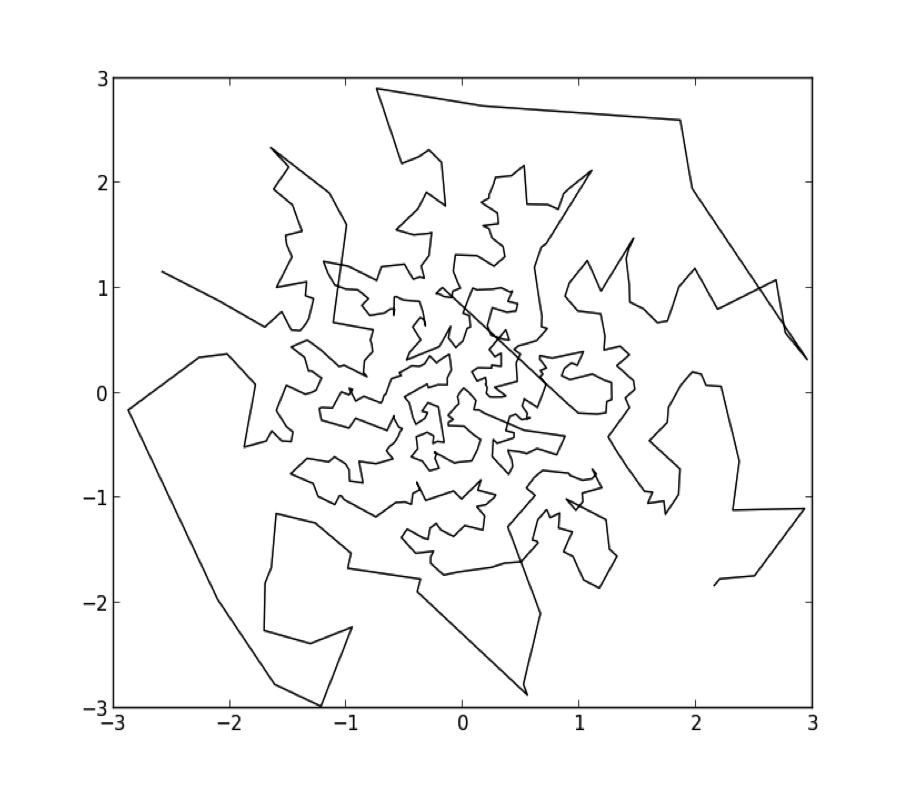
\includegraphics[scale=.6]{6.png}\\
Greedy 3 optimization
\end{center}
\begin{center}
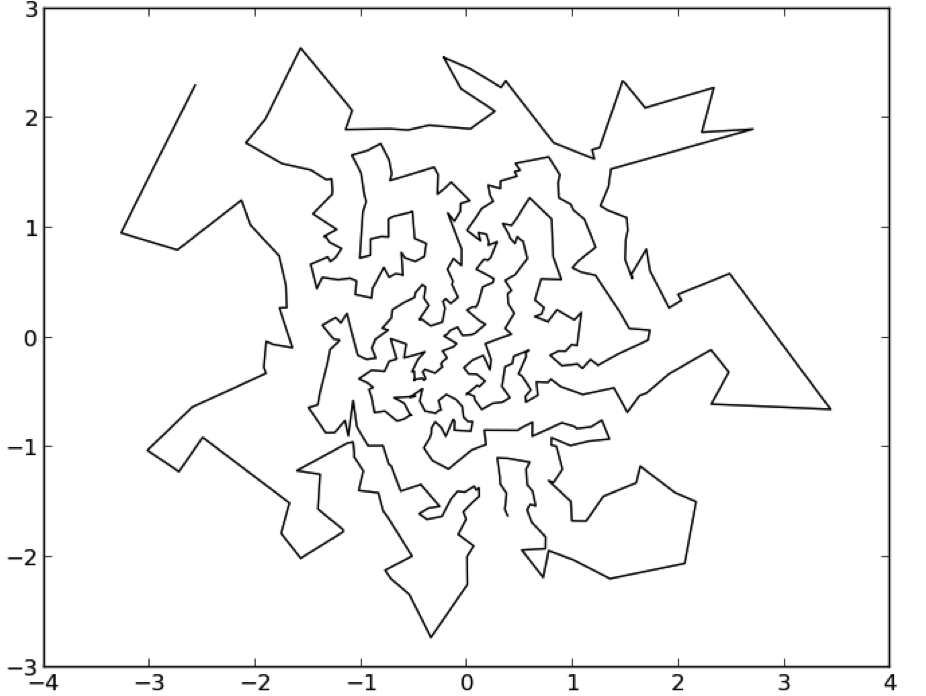
\includegraphics[scale=.6]{7.png}\\
Kocay's Algorithm, first node heuristic
\end{center}
\begin{center}
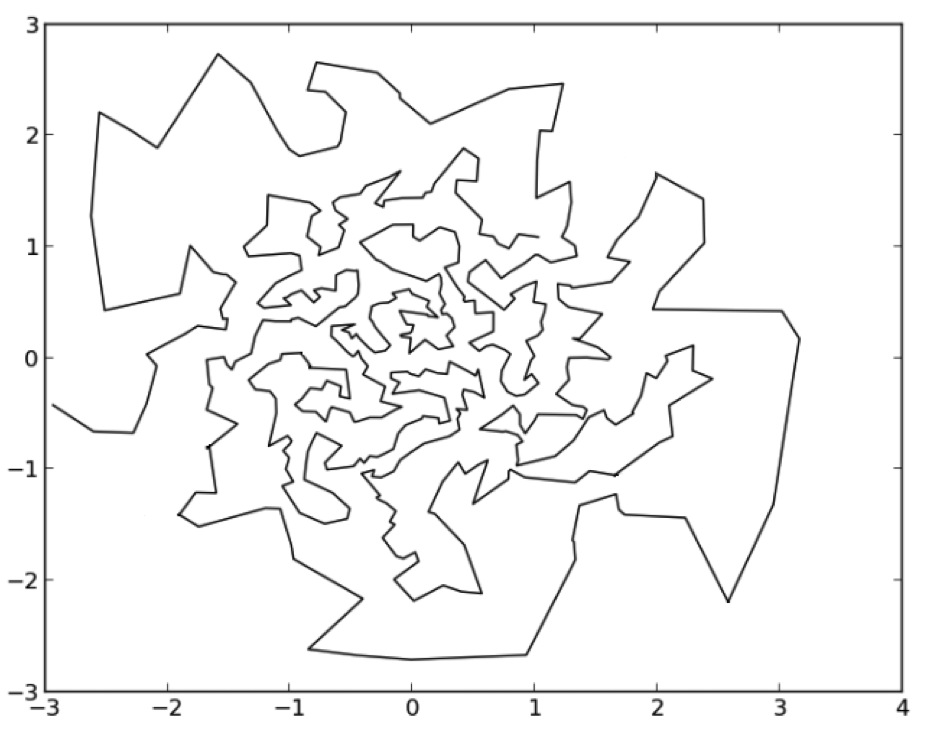
\includegraphics[scale=.6]{8.png}\\
Kocay's Algorithm, random node 
\end{center}

\section{References:}
[1] Krivelevich, M., Lee, C., & Sudakov, B. (2014). Compatible Hamilton cycles in Dirac graphs. arXiv preprint arXiv:1410.1435. \hfill \break
[2] Ferber, A., Nenadov, R., Noever, A., Peter, U., & Skoric, N. (2014). Robust hamiltonicity of random directed graphs. arXiv preprint arXiv:1410.2198. \hfill \break
[3] Sardroud, A. A., & Bagheri, A. (2015). An approximation algorithm for the longest cycle problem in solid grid graphs. arXiv preprint arXiv:1502.07085. \hfill \break
[4] Fukasawa, R., Barboza, A. S., & Toriello, A. (2015). A Comparison of Bounds for the Traveling Salesman Problem. \hfill \break
[5] Woods, B., Punnen, A., & Stephen, T. (2015). A Linear Time Algorithm for the $3 $-Neighbour Traveling Salesman Problem on Halin graphs and extensions. arXiv preprint arXiv:1504.02151. \hfill \break














\end{document}